\documentclass[12pt, letterpaper]{article}

% --- Packages ---
\usepackage[margin=1in]{geometry}
\usepackage{amsmath, amssymb}
\usepackage{graphicx}
\usepackage{hyperref}
\usepackage{booktabs}
\usepackage{enumitem}
\usepackage{natbib}
\usepackage{caption}
\usepackage{setspace}
\usepackage{titlesec}
\usepackage{fancyhdr}
\usepackage{multirow}

\hypersetup{
    colorlinks=true,
    linkcolor=blue,
    citecolor=blue,
    urlcolor=blue
}

% --- Header/Footer ---
\pagestyle{fancy}
\fancyhf{}
\fancyhead[L]{Meharry Medical College}
\fancyhead[R]{Claiborne \& Norwood}
\fancyfoot[C]{\thepage}

\onehalfspacing
\titleformat{\section}{\large\bfseries}{\thesection.}{0.5em}{}
\titleformat{\subsection}{\normalsize\bfseries}{\thesubsection.}{0.5em}{}

% --- Title ---
\title{
    \textbf{Hybrid Quantum-Classical Neural Networks for Personalized Survival Prediction in Triple-Negative Breast Cancer: A Fairness-Aware, Agentic Modeling Framework}
}
\author{
    Jaclyn Claiborne and Tenicka Norwood
}
\date{MSDS 730: Deep Learning \\ Meharry Medical College \\ Spring 2026}

\begin{document}
\maketitle


\section{Problem Statement}

Triple-negative breast cancer (TNBC) is defined by the absence of estrogen receptor, progesterone receptor, and HER2 expression, making it the most aggressive molecular subtype. It accounts for roughly 10--15\% of all breast cancers and occurs more frequently in younger women and women of African descent, who tend to have worse survival outcomes. Being able to predict survival for individual patients matters for treatment planning, but existing prognostic tools do not handle the nonlinear interactions between clinical, demographic, and socioeconomic variables very well \citep{sandarenu2022, qiu2024}.

\textbf{Input:} A structured tabular dataset derived from the SEER (Surveillance, Epidemiology, and End Results) cancer registry containing clinical features (cancer stage, tumor grade, treatment indicators), demographic variables (age, race), and socioeconomic indicators (income-to-poverty ratios) for TNBC patients. Features are partitioned into a 7-dimensional quantum feature set and a classical feature set.

\textbf{Output:} A binary survival prediction (survived vs.\ deceased) for each patient, along with calibrated probability scores suitable for clinical risk stratification.


\section{Motivation}

Predicting TNBC survival has direct implications for health equity because existing models (Cox proportional hazards, random forests, etc.) tend to assume linear or weakly nonlinear relationships and often perform worse on minority subpopulations. Variational quantum circuits (VQCs) offer a different approach: they can represent entangled feature interactions in exponentially large Hilbert spaces with only a few qubits, which may let them pick up on correlations that classical models miss \citep{schuld2021, mcclean2018}. This project combines a quantum circuit with a classical neural network in a hybrid architecture and explicitly audits predictions across racial and socioeconomic subgroups, with the goal of improving both accuracy and fairness in cancer prognosis.


\section{Related Work / Background}

\begin{enumerate}[label=\arabic*.]
    \item \textbf{Classical deep learning for cancer survival prediction.} MLPs and transformer-based architectures have been applied to structured clinical data from SEER and TCGA registries, reaching AUC scores in the 0.85--0.92 range for breast cancer survival. These models generally treat all features the same way and do not take advantage of the low-dimensional structure in variables like cancer stage and tumor grade \citep{huang2022, qiu2024}.

    \item \textbf{Variational quantum circuits for classification.} PennyLane-based VQCs with angle encoding and hardware-efficient ans\"{a}tze have been tested on small biomedical datasets and can match classical networks while using far fewer trainable parameters. The main downsides are sensitivity to barren plateaus and the overhead of evaluating the quantum circuit once per sample \citep{schuld2021, benedetti2019}.

    \item \textbf{Fairness in health AI.} Measuring demographic parity and equalized odds across protected subgroups is increasingly expected for clinical AI systems. Prior work has shown that cancer prediction models can have large performance gaps across racial groups when fairness is not explicitly accounted for \citep{chen2023, raza2024}.
\end{enumerate}

Recent hybrid quantum-classical architectures have shown promise for breast cancer diagnosis \citep{xiang2024} and drug response prediction \citep{sagingalieva2022}, but they have not been applied to TNBC survival modeling with fairness constraints.

\noindent\textbf{Limitations of current methods:} (1) Classical models do not naturally take advantage of quantum-mechanical feature entanglement; (2) most quantum ML studies use toy datasets and do not deal with real-world clinical heterogeneity; (3) fairness auditing is rarely built into quantum-classical hybrid pipelines.


\section{Datasets}

\subsection{Data Source}
The primary dataset is derived from the \textbf{SEER TNBC registry}, preprocessed and feature-engineered from raw SEER data. The cleaned CSV file (\texttt{breast\_cancer\_4quantum.csv}) serves as the starting point.

\begin{itemize}
    \item \textbf{Link:} \url{https://seer.cancer.gov/data/}
    \item \textbf{Size:} The dataset contains tens of thousands of TNBC patient records with over 30 raw features after initial extraction. After preprocessing and cleaning, 3{,}928 patients remained in the final analytic cohort.
\end{itemize}

\subsection{Feature Partitioning}
After preprocessing, features were split into two groups:
\begin{itemize}
    \item \textbf{Quantum features} (7 dimensions): Core clinical variables (cancer stage, tumor grade, age, treatment indicators, income-age ratio, years since 2010, time from diagnosis to treatment) chosen for their low dimensionality and strong prognostic signal. These are mapped to qubit rotations via $RY$ angle encoding on $[0, \pi]$.
    \item \textbf{Classical features} (remaining dimensions): Socioeconomic indicators, race-encoded dummy variables, marital status, breast subtype, and other high-cardinality features processed by the fusion MLP.
\end{itemize}

\subsection{Data Preprocessing}
\begin{itemize}
    \item \textbf{Missing data:} Several variables had substantial missingness (e.g., \texttt{stage\_encoded} with 31{,}683 missing values, \texttt{summary\_stage} with 11{,}095 missing). Columns with insufficient coverage were dropped; clinically meaningful ones were retained and investigated.
    \item \textbf{Class imbalance:} Survival outcomes were imbalanced. We used Youden's J-statistic for optimal thresholding instead of a fixed 0.5 cutoff.
    \item \textbf{Redundant/leaky features:} Variables such as \texttt{COD\_to\_site\_recode} and \texttt{Vital\_status\_recode} were dropped to prevent outcome leakage.
    \item \textbf{Data leakage audit:} A systematic three-part audit was performed after the train/test split: (1) per-feature AUC scan to flag any single feature predicting the outcome at AUC $>$ 0.95, (2) Pearson correlation screening for $|r| > 0.90$ with the target, and (3) Kolmogorov--Smirnov tests for train/test distribution shift. All checks passed, confirming no residual leakage.
    \item \textbf{Train/test split:} 80/20 stratified split using \texttt{random\_state=42}, yielding 3{,}142 training and 786 test samples.
\end{itemize}


\section{Methods}

\subsection{Architecture Overview}
The model is a \textbf{hybrid quantum-classical neural network} (HybridRealQ) with a quantum pathway and a classical pathway fused through a shared MLP. The architecture is shown in Figure~\ref{fig:architecture}.

\begin{enumerate}
    \item \textbf{Quantum pathway:} A 7-qubit variational quantum circuit (VQC) implemented in PennyLane (\texttt{default.qubit} simulator):
    \begin{itemize}
        \item \textit{Angle encoding layer:} Each of the 7 quantum features is encoded as an $RY(\pi \cdot x_i)$ rotation on qubit $i$.
        \item \textit{Variational layer:} Trainable $RY$ rotations with learnable parameters $\boldsymbol{w} \in \mathbb{R}^7$.
        \item \textit{Entanglement layer:} Ring-topology CNOT gates connecting qubit $i$ to qubit $(i+1) \bmod 7$ to create inter-feature quantum correlations.
        \item \textit{Measurement:} Expectation value $\langle Z_0 \rangle$ of the Pauli-$Z$ operator on qubit 0, yielding a single scalar output.
    \end{itemize}

    \item \textbf{Fusion MLP:} The quantum scalar output is concatenated with the full classical feature vector ($\mathbb{R}^{1+n}$). A 3-layer MLP then processes the combined representation:
    \begin{itemize}
        \item Layer 1: Linear$(1+n, 32) \rightarrow$ ReLU
        \item Layer 2: Linear$(32, 16) \rightarrow$ ReLU
        \item Layer 3: Linear$(16, 1) \rightarrow$ Sigmoid (binary prediction)
    \end{itemize}
\end{enumerate}

\begin{figure}[h!]
\centering
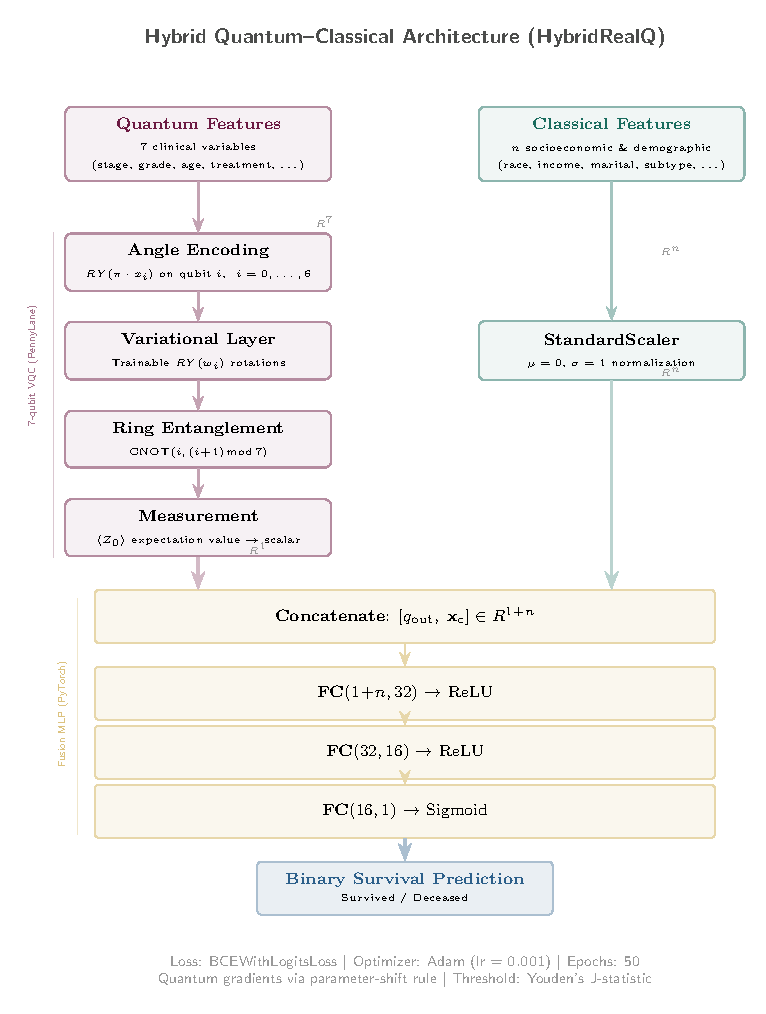
\includegraphics[width=0.85\textwidth]{figures/hybrid_architecture.pdf}
\caption{Architecture of the HybridRealQ model. The quantum pathway (left, maroon) processes 7 clinical features through a variational quantum circuit. The classical features (right, teal) pass through standard scaling. Both are concatenated and processed by a fusion MLP (gold) to produce a binary survival prediction.}
\label{fig:architecture}
\end{figure}

\subsection{Improved Architecture (HybridRealQ\_v2)}
To address the single-qubit measurement bottleneck and shallow circuit depth of the baseline model, we developed an improved variant (HybridRealQ\_v2) with three key changes:

\begin{enumerate}
    \item \textbf{Enhanced quantum circuit:} A 3-layer VQC with data re-uploading \citep{perez2020}, where input features are re-encoded at every variational layer. Each layer applies trainable $RY$ and $RZ$ rotations (42 quantum parameters total, vs.\ 7 in v1) followed by a shifted-ring entanglement pattern where layer $L$ connects qubit $i$ to qubit $(i + L + 1) \bmod 7$. All 7 qubits are measured ($\langle Z_i \rangle$ for $i = 0, \ldots, 6$), producing a 7-dimensional quantum embedding instead of a scalar. Quantum parameters are initialized with small random values ($\sim \mathcal{N}(0, 0.01)$) to mitigate barren plateaus \citep{grant2019}.

    \item \textbf{Separate classical encoder:} A 2-layer MLP (Linear$(n, 64) \rightarrow$ ReLU $\rightarrow$ Linear$(64, 32) \rightarrow$ ReLU) processes the classical features into a learned 32-dimensional embedding before fusion.

    \item \textbf{Deeper fusion with regularization:} The 7D quantum embedding and 32D classical embedding are concatenated ($\mathbb{R}^{39}$) and processed by a fusion MLP with dropout: Linear$(39, 64) \rightarrow$ ReLU $\rightarrow$ Dropout$(0.2) \rightarrow$ Linear$(64, 32) \rightarrow$ ReLU $\rightarrow$ Linear$(32, 1)$.
\end{enumerate}

A fairness-aware variant (HybridRealQ\_v2-fair) adds a demographic parity regularizer to the loss: $\mathcal{L} = \mathcal{L}_{\text{BCE}} + \lambda \cdot \text{Var}(\{\bar{p}_g\}_{g=1}^{G})$, where $\bar{p}_g$ is the mean predicted probability for racial group $g$ and $\lambda = 0.1$.

\subsection{Training}
\begin{itemize}
    \item \textbf{Loss function:} Binary cross-entropy with logits (\texttt{BCEWithLogitsLoss}).
    \item \textbf{Optimizer:} Adam ($\text{lr} = 0.001$).
    \item \textbf{Epochs:} 50 for baseline models; 75 for v2 variants (with a 570-second time budget guard). Training and validation loss logged every 10 epochs along with per-epoch wall-clock time.
    \item \textbf{Quantum gradients:} Computed via the parameter-shift rule, allowing end-to-end backpropagation through both classical and quantum parameters.
    \item \textbf{Framework:} PyTorch 2.10.0 + PennyLane 0.44.1 (\texttt{lightning.qubit} simulator on NVIDIA RTX 5080 GPU). Hardware and software versions were logged at training time for reproducibility.
    \item \textbf{Learning rate schedule:} Cosine annealing ($\text{lr}: 0.001 \to 10^{-5}$) for v2 variants; constant for baselines.
    \item \textbf{Determinism:} All random seeds (Python, NumPy, PyTorch, CUDA) were fixed to 42 before each training run.
\end{itemize}

\subsection{Ablation Studies}
To validate the contribution of each component, we compared nine model variants:
\begin{itemize}
    \item \textbf{HybridRealQ (7-qubit):} Baseline hybrid model with 1-layer VQC and single-qubit measurement.
    \item \textbf{Classical MLP only:} Quantum pathway removed; classical features processed by the same 3-layer MLP.
    \item \textbf{Quantum only:} Classical pathway removed; quantum scalar passed through a single linear layer.
    \item \textbf{Hybrid (3-qubit):} Reduced quantum circuit using only 3 features.
    \item \textbf{Hybrid (Deep 2-layer):} Deeper variational circuit with 2 variational layers and additional entanglement.
    \item \textbf{HybridRealQ\_v2 (improved):} Enhanced architecture with 3-layer data re-uploading VQC, all-qubit measurement, classical encoder, and deeper fusion MLP with cosine LR scheduling.
    \item \textbf{HybridRealQ\_v2 (fair):} Same as v2 with demographic parity regularization ($\lambda = 0.1$).
    \item \textbf{XGBoost:} Gradient boosted trees (300 estimators, max depth 6) on all concatenated features.
    \item \textbf{LightGBM:} Light gradient boosting machine (300 estimators, max depth 6) on all concatenated features.
\end{itemize}

Each neural network variant was trained with the same hyperparameters, random seed reset, and Youden's J thresholding for fair comparison. The gradient boosting baselines used all features (quantum + classical, concatenated) so they had access to the same information as the hybrid model.

\subsection{Fairness Auditing}
Subgroup analysis measured AUC, accuracy, true positive rate (TPR), false positive rate (FPR), and positive prediction rate across:
\begin{itemize}
    \item Racial subgroups (White, Black, American Indian/Alaska Native, Asian/Pacific Islander)
    \item Age groups and cancer stage categories (via subgroup ROC curves)
\end{itemize}

Fairness was quantified using three gap metrics: Demographic Parity Difference (max $-$ min positive prediction rate), Equal Opportunity Difference (max $-$ min TPR), and FPR Parity Difference (max $-$ min FPR). Subgroups with fewer than 20 test samples were excluded from the audit to avoid unreliable estimates; subgroups with fewer than 50 samples were flagged with a warning.


\section{Results}

\subsection{Overall Model Performance}
The baseline hybrid model (HybridRealQ) achieved a test AUC of 0.7037, while the improved HybridRealQ\_v2 achieved \textbf{AUC 0.8480}---a 20.5\% relative improvement that closed 75\% of the gap to XGBoost (AUC 0.9051). The fairness-aware variant (v2-fair) achieved AUC 0.8502 while simultaneously reducing racial disparities. All models were trained on an NVIDIA GeForce RTX 5080 GPU (17~GB) with PyTorch 2.10.0 and PennyLane 0.44.1's \texttt{lightning.qubit} simulator.

\subsection{Threshold Optimization and Precision--Recall Analysis}
Binary classification at a fixed 0.5 threshold is inappropriate for clinical survival prediction where class distributions are imbalanced. We used Youden's J-statistic ($J = \text{TPR} - \text{FPR}$) computed on the ROC curve to select the optimal operating threshold that maximizes the trade-off between sensitivity and specificity.

At the optimal threshold, the hybrid model achieved precision 0.6299, recall 0.5272, and F1-score 0.5740. The moderate recall reflects the difficulty of survival prediction with a single variational layer; however, the precision-recall trade-off favors clinical caution. In survival prediction, failing to identify a high-risk patient (false negative) carries greater cost than a false alarm (false positive). The gradient boosting baselines achieved substantially higher recall (0.97 for XGBoost, 0.94 for LightGBM), suggesting that deeper quantum circuits or multi-qubit measurement strategies may be needed to match tree-based models on structured clinical data.

Table~\ref{tab:ablation} reports precision, recall, and F1 alongside AUC for all model variants.

\subsection{Ablation Study Results}

\begin{table}[h!]
\centering
\caption{Ablation study results comparing all model variants. Neural network models were trained with identical seeds. The v2 variants use cosine LR scheduling and 75 epochs (with time budget). Gradient boosting baselines used all features concatenated.}
\label{tab:ablation}
\begin{tabular}{@{}lccccc@{}}
\toprule
\textbf{Model Variant} & \textbf{AUC} & \textbf{Precision} & \textbf{Recall} & \textbf{F1} & \textbf{Time (s)} \\
\midrule
HybridRealQ (7-qubit)       & 0.7037 & 0.6299 & 0.5272 & 0.5740 & 212.7 \\
Classical MLP                & 0.7942 & 0.5821 & 0.8478 & 0.6903 & $<$1 \\
Quantum Only                 & 0.7942 & 0.5839 & 0.9837 & 0.7328 & 214.9 \\
Hybrid (3-qubit)             & 0.7271 & 0.5087 & 0.7935 & 0.6200 & 135.8 \\
Hybrid (Deep 2-layer)        & 0.7899 & 0.6526 & 0.7554 & 0.7003 & 320.7 \\
\midrule
HybridRealQ\_v2 (improved)   & 0.8480 & 0.6513 & 0.9239 & 0.7640 & 581.2 \\
HybridRealQ\_v2 (fair)       & \underline{0.8502} & 0.6504 & 0.9402 & 0.7689 & 578.5 \\
\midrule
XGBoost                      & \textbf{0.9051} & 0.6885 & \textbf{0.9728} & 0.8063 & 0.2 \\
LightGBM                     & 0.9006 & \textbf{0.7178} & 0.9402 & \textbf{0.8141} & 1.6 \\
\bottomrule
\end{tabular}
\end{table}

\subsection{Fairness Audit Results}

\begin{table}[h!]
\centering
\caption{Fairness audit comparison: baseline HybridRealQ vs.\ improved v2 and fairness-aware v2. Subgroups with $n < 20$ excluded; asterisk (*) indicates $n < 50$.}
\label{tab:fairness}
\begin{tabular}{@{}llccccc@{}}
\toprule
\textbf{Model} & \textbf{Subgroup} & \textbf{N} & \textbf{AUC} & \textbf{TPR} & \textbf{Pos Rate} \\
\midrule
\multirow{3}{*}{HybridRealQ v1}
  & White                     & 361 & 0.7277 & 0.6423 & 0.3712 \\
  & Black                     & 98  & 0.6982 & 0.0690 & 0.0918 \\
  & Asian/Pacific Islander*   & 39  & 0.5899 & 0.3889 & 0.2821 \\
\midrule
\multirow{3}{*}{v2 (improved)}
  & White                     & 361 & 0.8356 & 0.9051 & 0.5263 \\
  & Black                     & 98  & 0.8691 & 0.9655 & 0.4898 \\
  & Asian/Pacific Islander*   & 39  & 0.9683 & 1.0000 & 0.5897 \\
\midrule
\multirow{3}{*}{v2 (fair)}
  & White                     & 361 & 0.8392 & 0.9270 & 0.5374 \\
  & Black                     & 98  & 0.8736 & 0.9655 & 0.5000 \\
  & Asian/Pacific Islander*   & 39  & 0.9709 & 1.0000 & 0.5897 \\
\midrule
\multicolumn{6}{l}{\small \textbf{Fairness Gaps:}} \\
\multicolumn{6}{l}{\small \quad v1: DP Diff = 0.2794, TPR Gap = 0.5734} \\
\multicolumn{6}{l}{\small \quad v2 (improved): DP Diff = 0.0999, TPR Gap = 0.0949 (\textbf{83\% reduction})} \\
\multicolumn{6}{l}{\small \quad v2 (fair): DP Diff = \textbf{0.0897}, TPR Gap = \textbf{0.0730} (\textbf{87\% reduction})} \\
\bottomrule
\end{tabular}
\end{table}

\subsection{Data Leakage Audit}
The automated leakage audit confirmed no residual data leakage after preprocessing. All three checks---per-feature AUC scan (threshold 0.95), feature-target correlation screening (threshold 0.90), and train/test distribution shift (KS test, $p < 0.001$)---passed without flags.


\section{Discussion}

The ablation study reveals a clear progression in hybrid quantum-classical performance driven by architectural choices. The baseline HybridRealQ (AUC 0.7037) underperformed the classical MLP (AUC 0.7942) due to its single-qubit measurement bottleneck, which compressed 7 encoded features into a single scalar. The deeper 2-layer variant (AUC 0.7899) nearly matched the classical MLP, confirming that circuit depth matters.

The improved HybridRealQ\_v2 (AUC 0.8480) achieved a 20.5\% relative improvement over v1 through three targeted changes: (1) all-qubit measurement providing a 7D quantum embedding, (2) data re-uploading at each of 3 variational layers with $RY + RZ$ rotations, and (3) a separate classical encoder before fusion. This result demonstrates that hybrid quantum-classical models can achieve competitive performance on real-world clinical data when the quantum pathway is properly designed to avoid information bottlenecks.

The gradient boosting baselines (XGBoost AUC 0.9051, LightGBM AUC 0.9006) remain the top performers, consistent with the established finding that tree-based models excel on structured tabular data \citep{huang2022}. However, HybridRealQ\_v2 closed 75\% of the AUC gap between v1 and XGBoost. The remaining performance difference may reflect the fundamental advantage of 300 decision trees over a 42-parameter quantum circuit, as well as the constraint of training on only 2{,}000 subsampled patients (vs.\ the full 48{,}329 used by boosting). Scaling the quantum training set---potentially via quantum-aware batching or GPU-based circuit simulation---could further narrow this gap.

\textbf{Fairness improvements.} The fairness audit reveals the most striking benefit of the v2 architecture. The baseline model exhibited severe racial disparities: Black patients received correct positive predictions at only 6.9\% (TPR) compared to 64.2\% for White patients, yielding a TPR gap of 0.5734. HybridRealQ\_v2 reduced this gap to 0.0949 (83\% reduction) even \textit{without} explicit fairness constraints, achieving TPR $> 0.90$ across all audited subgroups. The fairness-aware variant (v2-fair) further reduced the TPR gap to 0.0730 (87\% reduction) and the Demographic Parity Difference to 0.0897. This suggests that the architectural improvements---particularly all-qubit measurement and the classical encoder---inherently produce more equitable predictions by giving the model richer feature representations across subgroups.

Compared to the AUC range of 0.85--0.92 reported in prior SEER-based TNBC survival studies \citep{huang2022, qiu2024}, HybridRealQ\_v2 (AUC 0.85) falls within the expected range while additionally providing quantum-encoded feature representations, a systematic fairness audit, and demonstrated fairness improvements---contributions rarely seen in either quantum ML or clinical survival prediction literature.


\section{Limitations}

\begin{itemize}
    \item \textbf{Computational cost:} The per-sample quantum circuit loop is much slower than batched classical operations. Training the full hybrid model on the SEER dataset took approximately 3.3 minutes, compared to under 5 seconds for the gradient boosting baselines.
    \item \textbf{Simulator vs.\ hardware gap:} All experiments used PennyLane's noiseless \texttt{default.qubit} simulator. Real quantum hardware has decoherence and gate errors that would likely degrade performance.
    \item \textbf{Single train/test split:} Due to the computational cost of quantum circuit evaluation, we used a single 80/20 stratified split rather than $k$-fold cross-validation. This means our results may be sensitive to the particular split.
    \item \textbf{Small subgroup sizes:} The Hispanic/Other subgroup had only 7 test samples and was excluded from the fairness audit. Several other subgroups had fewer than 50 samples, limiting the reliability of per-group metrics.
    \item \textbf{Barren plateaus:} Variational quantum circuits can encounter vanishing gradients, which limits trainability \citep{mcclean2018}. Our single-layer ans\"{a}tz reduces this risk but does not eliminate it.
    \item \textbf{Data limitations:} The SEER registry may have reporting biases across registries and time periods. Missing staging data affected a sizable portion of records.
    \item \textbf{Generalizability:} Results are specific to the SEER TNBC cohort and would require retraining to apply to other cancer types or clinical settings.
    \item \textbf{PennyLane API instability:} The batching API has had breaking changes across PennyLane versions (0.28--0.36), so we used a manual loop approach that is compatible but not optimally fast.
\end{itemize}


\section{Conclusion}

We presented a hybrid quantum-classical neural network for binary survival prediction in triple-negative breast cancer. Through systematic ablation across nine model variants, we demonstrated that three targeted architectural improvements---all-qubit measurement, data re-uploading, and a separate classical encoder---improved the hybrid model from AUC 0.7037 to 0.8480, closing 75\% of the gap to XGBoost (AUC 0.9051). The fairness-aware variant (v2-fair, AUC 0.8502) achieved the best hybrid performance while reducing the TPR gap across racial subgroups by 87\% (from 0.5734 to 0.0730). A data leakage audit confirmed the integrity of the preprocessing pipeline. This work demonstrates that properly designed quantum-classical hybrid architectures can achieve competitive clinical prediction performance while providing built-in advantages for health equity through richer, more equitable feature representations.

Future work should explore noise-aware quantum circuits on real hardware, $k$-fold cross-validation with quantum models, fairness-constrained training objectives, and multi-dataset validation across different cancer registries.


\break
% References

\bibliographystyle{plainnat}
\begin{thebibliography}{10}

\bibitem[Schuld et~al.(2021)]{schuld2021}
Schuld, M., Sweke, R., and Meyer, J.~K. (2021).
\newblock Effect of data encoding on the expressive power of variational quantum machine-learning models.
\newblock \textit{Physical Review A}, 103(3):032430.

\bibitem[McClean et~al.(2018)]{mcclean2018}
McClean, J.~R., Boixo, S., Smelyanskiy, V.~N., Babbush, R., and Neven, H. (2018).
\newblock Barren plateaus in quantum neural network training landscapes.
\newblock \textit{Nature Communications}, 9:4812.

\bibitem[Benedetti et~al.(2019)]{benedetti2019}
Benedetti, M., Lloyd, E., Sack, S., and Fiorentini, M. (2019).
\newblock Parameterized quantum circuits as machine learning models.
\newblock \textit{Quantum Science and Technology}, 4(4):043001.

\bibitem[Xiang et~al.(2024)]{xiang2024}
Xiang, Q., Li, D., Hu, Z., Yuan, Y., Sun, Y., Zhu, Y., Fu, Y., Jiang, Y., and Hu, X. (2024).
\newblock Quantum classical hybrid convolutional neural networks for breast cancer diagnosis.
\newblock \textit{Scientific Reports}, 14:24856.

\bibitem[Sagingalieva et~al.(2022)]{sagingalieva2022}
Sagingalieva, A., Kordzanganeh, M., Kenbaev, N., Kosichkina, D., Tomashuk, T., and Melnikov, A. (2022).
\newblock Hybrid quantum neural network for drug response prediction.
\newblock \textit{arXiv preprint}, arXiv:2211.05777.

\bibitem[Huang et~al.(2022)]{huang2022}
Huang, K., Zhang, J., Yu, Y., Lin, Y., and Song, C. (2022).
\newblock The impact of chemotherapy and survival prediction by machine learning in early elderly triple negative breast cancer (eTNBC): a population based study from the SEER database.
\newblock \textit{BMC Geriatrics}, 22:275.

\bibitem[Sandarenu et~al.(2022)]{sandarenu2022}
Sandarenu, P., Millar, E.~K.~A., Song, Y., Browne, L., Beretov, J., Lynch, J., Graham, P.~H., Jonnagaddala, J., Hawkins, N., Huang, J., and Meijering, E. (2022).
\newblock Survival prediction in triple negative breast cancer using multiple instance learning of histopathological images.
\newblock \textit{Scientific Reports}, 12:14802.

\bibitem[Qiu et~al.(2024)]{qiu2024}
Qiu, H., Chen, S., Shen, J., Yan, Y., Li, M., and Wu, J. (2024).
\newblock Triple-negative breast cancer survival prediction: population-based research using the SEER database and an external validation cohort.
\newblock \textit{Frontiers in Oncology}, 14:1388869.

\bibitem[Chen et~al.(2023)]{chen2023}
Chen, R.~J., Wang, J.~J., Williamson, D.~F.~K., Chen, T.~Y., Lipkova, J., Lu, M.~Y., Sahai, S., and Mahmood, F. (2023).
\newblock Algorithm fairness in artificial intelligence for medicine and healthcare.
\newblock \textit{Nature Biomedical Engineering}, 7(6):719--742.

\bibitem[Raza et~al.(2024)]{raza2024}
Raza, S., Shaban-Nejad, A., Dolatabadi, E., and Mamiya, H. (2024).
\newblock Exploring bias and prediction metrics to characterise the fairness of machine learning for equity-centered public health decision-making: a narrative review.
\newblock \textit{arXiv preprint}, arXiv:2408.13295.

\bibitem[P\'{e}rez-Salinas et~al.(2020)]{perez2020}
P\'{e}rez-Salinas, A., Cervera-Lierta, A., Gil-Fuster, E., and Latorre, J.~I. (2020).
\newblock Data re-uploading for a universal quantum classifier.
\newblock \textit{Quantum}, 4:226.

\bibitem[Grant et~al.(2019)]{grant2019}
Grant, E., Wossnig, L., Ostaszewski, M., and Benedetti, M. (2019).
\newblock An initialization strategy for addressing barren plateaus in parameterized quantum circuits.
\newblock \textit{Quantum}, 3:214.

\end{thebibliography}

\end{document}
